% Theme stuff
\documentclass[xcolor=dvipsnames]{beamer}
%\documentclass[xcolor=dvipsnames,aspectratio=169]{beamer}
\usepackage{wasysym}
\usetheme{ScottLogic}

\title{AWSome fun in Amazon Web Services}
\date{\today}

\begin{document}

\begin{frame}
\titlepage
\end{frame}

\section*{Outline}
\subsection*{Overview}
\begin{frame}{Overview}
  \tableofcontents[hideallsubsections]
\end{frame}

\subsection*{Who's this for}
\begin{frame}{Who's this for}
  \begin{itemize}
    \item If you already know about...
    \begin{itemize}
      \item Vagrant
      \item Terraform
      \item Automation of cloud infrastructure
    \end{itemize}
    \item ...then you're not likely to get much out of this talk
    \pause
    \begin{itemize}
      \item but you may be able to point out our mistakes \smiley
    \end{itemize}
  \end{itemize}
\end{frame}


\section{Review}
\subsection{Project goal}
\begin{frame}{Project goal}
  \begin{block}{Goal}
    Investigate the different clustering strategies and performance of
    Cassandra and MariaDB.
  \end{block}
  \pause
  \begin{itemize}
    \item See James' talk for discussion of these databases
    \item Here concentrate on how we automated provisioning of the clusters
  \end{itemize}
\end{frame}

\subsection{Previous work}
\begin{frame}{Previous work}
  \begin{itemize}
    \item Dave and Laurie - single node comparison
    \item Docker containers running in an Ubuntu VM
    \item Manual setup of the VM
  \end{itemize}
\end{frame}

\subsection{Our aims}
\begin{frame}{Our aims}
  \begin{itemize}
    \item Move each database node to its own VM
    \item Initially running locally, later in AWS
    \item Automate setup of VMs - reproducibility, ease of use
    \item Get to play with various cloud orchestation tools \smiley
  \end{itemize}
\end{frame}


\section[Vagrant]{Vagrant - from local VMs to AWS}

\subsection{Overview of Vagrant}
\begin{frame}{Vagrant overview}
  \begin{block}{}
    \begin{quote}
      Create and configure lightweight, reproducible, and portable development environments

      \small{\hfill vagrantup.com}
    \end{quote}
  \end{block}
  \pause
  \begin{itemize}
    \item Ruby-based, procedural framework
    \item Flexible
    \begin{itemize}
      \item Multiple providers: VirtualBox, AWS, Docker...
      \item Multiple provisioners: Shell, Chef, Ansible...
    \end{itemize}
  \end{itemize}
\end{frame}

\subsection{Moving to multiple VMs}
\begin{frame}[fragile]{Moving to multiple VMs with Vagrant}
  \begin{itemize}
    \item Two Ubuntu-based VMs, one per database
    \item Vagrant handles networking
    \item Provisioned via shell scripts
    \item Push button process - all handled from Vagrant
    \pause
    \begin{block}{To spin up a cluster}
      \begin{verbatim}
        vagrant up\end{verbatim}
    \end{block}
    \item Downloads Ubuntu box, creates and provisions two VMs
  \end{itemize}
\end{frame}

\begin{frame}[fragile]{Snippet to provision a seed Cassandra node}
  \begin{block}{Vagrantfile}
  \begin{code}{ruby}
Vagrant.configure("2") do |config|
  config.vm.provider "virtualbox" do |vb, vbconfig|
    vbconfig.vm.box = "ubuntu/xenial64"
    vb.memory       = 1024
    vbconfig.vm.network "private_network", ip: private_ip
  end

  (cassandra_nodes + maria_nodes).each_with_index do |name, index|
    config.vm.define name do |node|
      node.vm.provision "shell", path: "cassandra/bootstrap.sh"
    end
  end
end
  \end{code}
  \end{block}
\end{frame}

\subsection[Cloudy time]{Moving into AWS}
\begin{frame}[fragile]{Extra AWS stuff}
  \begin{itemize}
    \item Moving to AWS is simple...
    \begin{block}{Vagrantfile - with AWS provider}
      \begin{code}{ruby}
node.vm.provider "aws" do |aws, awsconfig|
  awsconfig.vm.box     = "dummy"
  awsconfig.vm.box_url = "https://github.com/mitchellh/vagrant-aws/raw/master/dummy.box"

  # VM details
  aws.ami                = "ami-57eae033" # Ubuntu Server 16.04
  aws.region             = "eu-west-2"
  aws.instance_type      = "t2.micro"
  aws.subnet_id          = AWS_SUBNET_ID
  aws.security_groups    = [AWS_SECURITY_GROUP_ID]
end
      \end{code}
    \end{block}
  \end{itemize}
\end{frame}

\begin{frame}{Extra AWS stuff - downsides}
BUT
  \begin{itemize}
    \item Lots more manual setup
    \item Security group, keys
    \item As complexity grows, awkward to express dependencies
  \end{itemize}
\end{frame}

\section[Terraform]{Terraform - declarative language for infrastructure}

\subsection[Motivation]{Motivation for using Terraform}
\begin{frame}{Choose Terraform}
  \begin{itemize}
    \item Same people as Vagrant
    \item Easy to setup required AWS resources
    \item Handles dependencies for you
    \begin{itemize}
      \item e.g. test client needs to know IPs of database nodes
    \end{itemize}
  \end{itemize}
\end{frame}

\begin{frame}[fragile]{Terraform dependency handling}
  \begin{block}{cluster.tf}
    \begin{code}{ruby}
module "test-client" {
  <@source               = "../resources/cluster/test-client"
  ami                  = "${var.test-client_ami}"
  key_name             = "${var.key_name}"
  mariadb_password     = "${var.mariadb_password}"
  security_group_name  = "${var.security_group_name}"
  private_key          = "${var.private_key}"
  cluster_name         = "${var.cluster_name}"@>
  cassandra_primary_ip = "${module.cassandra.primary_ip}"
  mariadb_ips          = "${join(",", module.mariadb.private_ips)}"
}
    \end{code}
  \end{block}
\end{frame}

\subsection{Advantages}
\begin{frame}{Other advantages}
  \begin{itemize}
    \item Handles dependencies between VMs nicely
    \item Declarative - only makes changes needed
    \item Easy to modularise code
  \end{itemize}
\end{frame}

\subsection{Horrors}
\begin{frame}{Minor horrors}
  \begin{itemize}
    \item Immature - latest version 0.8.5 at time of writing
    \item Not meant for provisioning...
    \item Rubbish errors
    \pause
    \begin{block}{Example error message}
      \texttt{Script failed with error code 1}
    \end{block}
    \item What script? What nodes?
    \item Missing functionality
    \begin{itemize}
      \item Can't loop over modules
      \item Doesn't delete VMs after AMI creation
    \end{itemize}
  \end{itemize}
\end{frame}


\section[Mistakes / next steps]{Self-inflicted horrors / next steps}
\subsection{Horrors}
\begin{frame}{Self-inflicted horrors}
\begin{itemize}
  \item Using Terraform for provisioning - spaghettified mess of shell scripts
  \item Be wary of AWS free tier - easy to go beyond free hours with lots of VMs!
\end{itemize}
\pause
\begin{columns}
  \centering
  \begin{column}{0.5\textwidth}
    \begin{block}{Oops...}
      \centering
      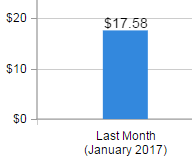
\includegraphics[width=0.7\textwidth]{AWSbilling.png}
    \end{block}
  \end{column}
\end{columns}
\end{frame}

\subsection{Next steps}
\begin{frame}{Next steps?}
  \begin{itemize}
    \item Use 'proper' provisioning solution?
    \item Try Chef for [infrastructure and] provisioning
    \begin{itemize}
      \item Lots of recipes available for Galera / Cassandra clusters
    \end{itemize}
  \end{itemize}
\end{frame}

\section{Summary}
\begin{frame}{Summary}
  \begin{itemize}
    \item We played about with lots of automation tools
    \item Vagrant is nice for simple independent dev environments
    \item Terraform is nice for cloud environments with lots of dependencies...
    \item ...but don't use it for provisioning
    \item Would be nice to know how it compares against more mature solutions
  \end{itemize}
\end{frame}

\end{document}
